\chapter{Variational Recurrent Neural Network}\label{sec:VRNN}

The \gls{vrnn} is the most expressive \gls{dvae}, in that sense that the general expressions \ref{gen_model_dvae}, \ref{inf_model_dvae} and \gls{vlb} \ref{vlb_dvae} can not be simplified.

The \gls{gpm} of the \gls{vrnn} assumes full connections between latent variables, and between observed variables, to account for the full unsimplified expressions. Specifically:

\begin{figure}[h]
    \centering
    % \includegraphics[width=0.5\linewidth]{}
    \label{fig:graphical_model_vrnn}
\begin{tikzpicture}[
    HIDDEN/.style={circle, draw=black!0, thin, minimum size=10mm},
    UNOBS/.style={circle, draw=black!80, thin, minimum size=10mm},
    OBS/.style={circle, draw=black!80, fill=gray!50, thin, minimum size=10mm}
]
% nodes
\node[HIDDEN] (zs) {$...$}; % start z
\node[HIDDEN] (xs) [below= of zs] {$...$}; % start x
\node[UNOBS] (z_t_1) [right= of zs] {$z_{t-1}$} edge[<-, thin] (a);
\node[OBS] (x_t_1) [below= of z_t_1] {$x_{t-1}$}    edge[<-, thin] (z_t_1)
                                                    edge[<-, thin] (xs);
\node[UNOBS] (z_t)  [right= of z_t_1] {$z_{t}$} edge[<-, thin] (z_t_1)
                                                edge[<-, thin] (x_t_1);
\node[OBS] (x_t) [below= of z_t] {$x_{t}$}  edge[<-, thin] (z_t)
                                            edge[<-, thin] (x_t_1)
                                            edge[<-, thin] (z_t_1);
\node[UNOBS] (z_t_p1) [right= of z_t] {$z_{t+1}$}   edge[<-, thin] (z_t)
                                                    edge[<-, thin] (x_t);
\node[OBS] (x_t_p1) [below= of z_t_p1] {$x_{t+1}$}  edge[<-, thin] (z_t_p1)
                                                    edge[<-, thin] (x_t)
                                                    edge[<-, thin] (z_t);
\node[HIDDEN] (ze) [right= of z_t_p1] {$...$} edge[<-, thin] (z_t_p1); % end z
\node[HIDDEN] (xe) [right= of x_t_p1] {$...$} edge[<-, thin] (x_t_p1); % end x

\path[->]   (z_t_1) edge [bend left=+45] node[mid left] {} (z_t_p1)
            (x_t_1) edge [bend left=-45] node[mid left] {} (x_t_p1);
\end{tikzpicture}
\caption{Probabilistic model of a Variational RNN}
\end{figure}

We remember that:
\begin{align*}
    p(x_{1:T}, z_{1:T}) &= \prod_{t=1}^T p_{\theta_x}(x_t \vert x_{1:t-1}, z_{1:t}) p_{\theta_z}(z_t \vert x_{1:t-1}, z_{1:t-1})
\end{align*}

And posit Gaussian distributions with diagonal covariance and mean given by two networks:
\begin{align}
    p_{\theta_x}(x_t \vert x_{1:t-1}, z_{1:t}) &= \NNdiag{x_t}{\mu_{\theta_x}(x_{1:t-1}, z_{1:t})}{\sigma_{\theta_x}^2(x_{1:t-1}, z_{1:t})} \\
    p_{\theta_z}(z_t \vert z_{1:t-1}, x_{1:t-1}) &= \NNdiag{z_t}{\mu_{\theta_z}(z_{1:t-1}, x_{1:t-1})}{\sigma_{\theta_z}^2(z_{1:t-1}, x_{1:t-1})}
\end{align}

The true posterior being
\begin{align*}
    p(z_{1:T} \vert x_{1:T}) &= \prod_{t=1}^T p(z_t \vert z_{1:t-1}, x_{1:T})
\end{align*}
we choose the encoder with the same conditional dependencies and a Gaussian expression:
\begin{align*}
    q_{\phi}(z_{t} \vert z_{1:t-1}, x_{1:T}) &= \NNdiag{z_t}{\mu_{\phi}(z_{1:t-1}, x_{1:T})}{\sigma_{\phi}^2(z_{1:t-1}, x_{1:T})}
\end{align*}

The \gls{vlb} is:
\begin{align*}
    \VLB &= \sum_{t=1}^T \left[ \E{q_{\phi}(z_{1:t} \vert x_{1:T})} \log{p_{\theta_x}(x_t \vert x_{1:t-1}, z_{1:t})} - \E{q_{\phi}(z_{1:t-1} \vert x_{1:T})} \KL{q_{\phi}(z_t \vert z_{1:t-1}, x_{1:T})}{p_{\theta_z}(z_t \vert z_{1:t-1}, x_{1:t-1})}
    \right]
\end{align*}

As a summary
\begin{tcolorbox}[colback=blue!5!white,colframe=black!75!black,title=Variational RNN]
\begin{itemize}
    \item \textbf{generative model}
    \begin{align}
        \label{gen_model_vrnn}
        p_{\theta_x}(x_t \vert x_{1:t-1}, z_{1:t}) &= \NNdiag{x_t}{\mu_{\theta_x}(x_{1:t-1}, z_{1:t})}{\sigma_{\theta_x}^2(x_{1:t-1}, z_{1:t})} \\
        p_{\theta_z}(z_t \vert z_{1:t-1}, x_{1:t-1}) &= \NNdiag{z_t}{\mu_{\theta_z}(z_{1:t-1}, x_{1:t-1})}{\sigma_{\theta_z}^2(z_{1:t-1}, x_{1:t-1})}
    \end{align}
    \item \textbf{inference model}
    \begin{align}
        \label{inf_model_vrnn}
        q_{\phi}(z_{t} \vert z_{1:t-1}, x_{1:T}) &= \NNdiag{z_t}{\mu_{\phi}(z_{1:t-1}, x_{1:T})}{\sigma_{\phi}^2(z_{1:t-1}, x_{1:T})}
    \end{align}
    \item \textbf{\gls{vlb} for training}
    \begin{align}
        \label{vlb_vrnn}
        \begin{split}
        \VLB &= \sum_{t=1}^T  \E{q_{\phi}(z_{1:t} \vert x_{1:T})} \log{p_{\theta_x}(x_t \vert x_{1:t-1}, z_{1:t})} \\ &- \sum_{t=1}^T \E{q_{\phi}(z_{1:t-1} \vert x_{1:T})} \KL{q_{\phi}(z_t \vert z_{1:t-1}, x_{1:T})}{p_{\theta_z}(z_t \vert z_{1:t-1}, x_{1:t-1})}  \end{split}
    \end{align}
\end{itemize}
\end{tcolorbox}

We have chosen a different implementation from \cite{girin_dynamical_2022} and used three different \gls{lstm} networks to encode $z_{1:t}$, $x_{1:t-1}$ and $x_{t:T}$ respectively.

The PyTorch implementation is described below:


%
%
% ----- VARIATIONAL RNN ------------------
%
%

\newpage
\begin{landscape}
\begin{figure}
\begin{centering}
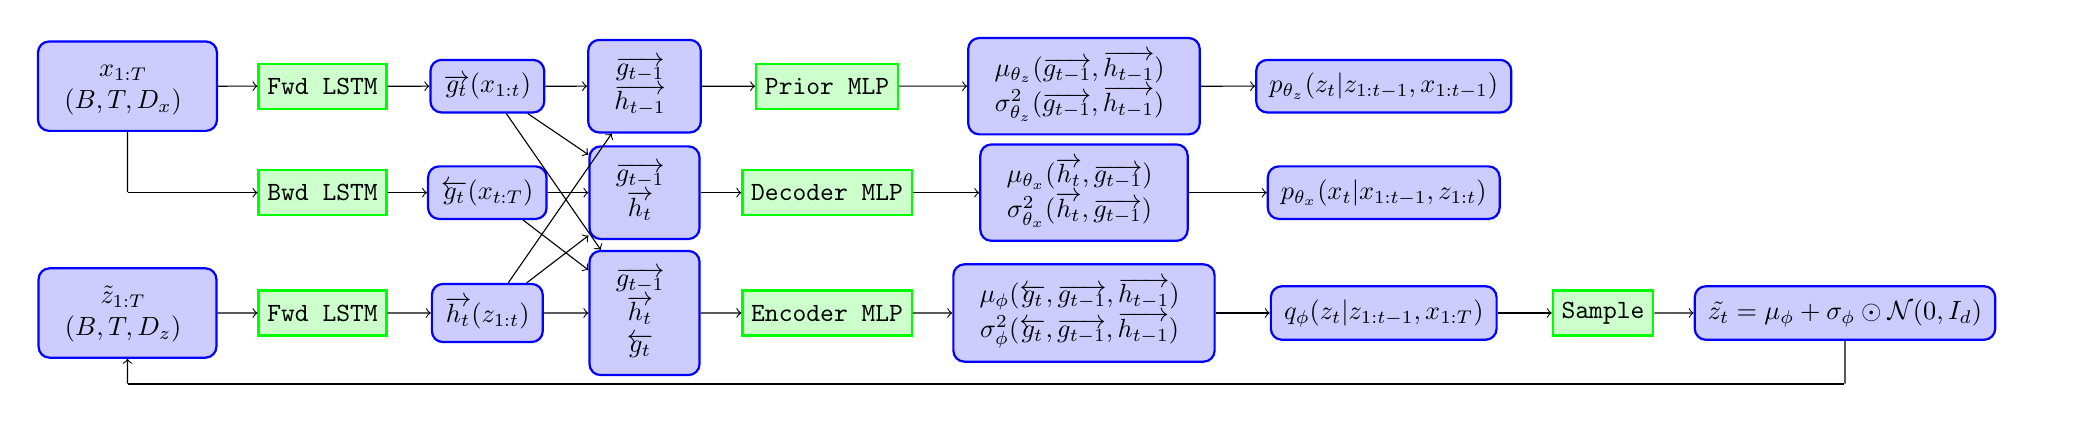
\begin{tikzpicture}[
    % format
    scale=0.95,
    every node/.style={scale=0.95},
    torch/.style={
        rectangle, 
        minimum size=6mm, 
        thick, 
        draw=green!100, 
        fill=green!20, 
        font=\ttfamily
        },
    math/.style={
        rectangle, 
        rounded corners, 
        thick, 
        draw=blue!100,
        fill=blue!20,
        align=center,
        anchor=center,
        inner sep=5pt
        },
    point/.style={
        circle,
        inner sep=0pt,
        minimum size=0pt,
        }
    ]
\matrix[row sep = 1mm, column sep=5mm] {
% row 1
\node[math] (xt) {
    $\begin{array}{c}
            x_{1:T} \\
            (B,T,D_x)
    \end{array}$
}; & 
\node[torch] (fwd_lstm) {Fwd LSTM}; & 
\node[math] (gt) {$\overrightarrow{g_t}(x_{1:t})$}; &
\node[math] (g_t_1_et_h_t_1) {
    $\begin{array}{c}
        \overrightarrow{g_{t-1}} \\
        \overrightarrow{h_{t-1}}
    \end{array}$
}; &
\node[torch] (prior) {Prior MLP}; &
\node[math] (theta_z) {
    $\begin{array}{c}
            \mu_{\theta_z}(\overrightarrow{g_{t-1}}, \overrightarrow{h_{t-1}}) \\
            \sigma_{\theta_z}^2(\overrightarrow{g_{t-1}}, \overrightarrow{h_{t-1}})
    \end{array}$
}; &
\node[math] (p_theta_z) {$p_{\theta_z}(z_t \vert z_{1:t-1}, x_{1:t-1})$}; & \\
% row 2
\node[point] (coin3) {}; &
\node[torch] (bwd_lstm) {Bwd LSTM}; & 
\node[math] (gt2) {$\overleftarrow{g_t}(x_{t:T})$}; &
\node[math] (g_t_1_et_h_t) {
    $\begin{array}{c}
        \overrightarrow{g_{t-1}} \\
        \overrightarrow{h_{t}}
    \end{array}$
}; &
\node[torch] (decoder) {Decoder MLP}; &
\node[math] (theta_x) {
    $\begin{array}{c}
            \mu_{\theta_x}(\overrightarrow{h_t}, \overrightarrow{g_{t-1}}) \\
            \sigma_{\theta_x}^2(\overrightarrow{h_t}, \overrightarrow{g_{t-1}})
    \end{array}$
}; & 
\node[math] (p_theta_x) {$p_{\theta_x}(x_t \vert x_{1:t-1}, z_{1:t} )$}; & \\
% row 3
\node[math] (z_tilde) {
    $\begin{array}{c}
            \tilde{z}_{1:T} \\
            (B,T,D_z)
    \end{array}$
}; & 
\node[torch] (fwd_lstm2) {Fwd LSTM}; & 
\node[math] (ht) {$\overrightarrow{h_t}(z_{1:t})$}; &
\node[math] (g_t_1_et_h_t_1_et_g_t) {
    $\begin{array}{c}
        \overrightarrow{g_{t-1}} \\
        \overrightarrow{h_{t}} \\
        \overleftarrow{g_t}
    \end{array}$
}; &
\node[torch] (encoder) {Encoder MLP}; &
\node[math] (phi) {
    $\begin{array}{c}
            \mu_{\phi}(\overleftarrow{g_{t}}, \overrightarrow{g_{t-1}}, \overrightarrow{h_{t-1}}) \\
            \sigma_{\phi}^2(\overleftarrow{g_{t}}, \overrightarrow{g_{t-1}}, \overrightarrow{h_{t-1}})
    \end{array}$
}; & 
\node[math] (q_phi) {$q_{\phi}(z_t \vert z_{1:t-1}, x_{1:T} )$}; &
\node[torch] (sample) {Sample}; &
\node[math] (z_tilde_formula) {$\tilde{z_t} = \mu_{\phi} + \sigma_{\phi} \odot \mathcal{N}(0, I_d)$}; & \\
% row 4
\node[point] (coin1) {};
& & & & & & & &;
\node[point] (coin2) {}; & \\
};
\path   (xt) edge [->, thin] (fwd_lstm)
        (xt) edge[-, thin] (coin3)
        (fwd_lstm) edge [->, thin] (gt)
        (gt) edge[->, thin] (g_t_1_et_h_t_1)
        (gt) edge[->, thin] (g_t_1_et_h_t)
        (gt) edge[->, thin] (g_t_1_et_h_t_1_et_g_t)
        (g_t_1_et_h_t_1) edge[->, thin] (prior)
        (prior) edge[->, thin] (theta_z)
        (theta_z) edge[->, thin] (p_theta_z)
        (coin3) edge[->, thin] (bwd_lstm)
        (bwd_lstm) edge[->, thin] (gt2)
        (gt2) edge[->, thin] (g_t_1_et_h_t)
        (gt2) edge[->, thin] (g_t_1_et_h_t_1_et_g_t)
        (g_t_1_et_h_t) edge[->, thin] (decoder)
        (decoder) edge[->, thin] (theta_x)
        (theta_x) edge[->, thin] (p_theta_x)
        (z_tilde) edge[->, thin] (fwd_lstm2)
        (fwd_lstm2) edge[->, thin] (ht)
        (ht) edge[->, thin] (g_t_1_et_h_t_1_et_g_t)
        (ht) edge[->, thin] (g_t_1_et_h_t)
        (ht) edge[->, thin] (g_t_1_et_h_t_1)
        (g_t_1_et_h_t_1_et_g_t) edge[->, thin] (encoder)
        (encoder) edge[->, thin] (phi)
        (phi) edge[->, thin] (q_phi)
        (q_phi) edge[->, thin] (sample)
        (sample) edge[->, thin] (z_tilde_formula)
        (z_tilde_formula) edge[-, thin] (coin2)
        (coin2) edge[-, thin] (coin1)
        (coin1) edge[->, thin] (z_tilde);
\end{tikzpicture}

% --- Loss VRNN
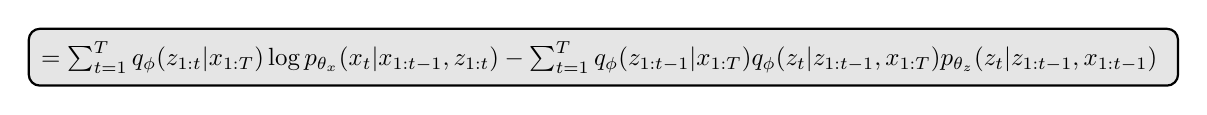
\begin{tikzpicture}[
    scale=0.90,
    every node/.style={scale=0.90},
    math/.style={
        rectangle, 
        % minimum height=1cm,
        % minimum width=2cm,
        rounded corners, 
        thick, 
        draw=black!100,
        fill=gray!20,
        align=center,
        anchor=center,
        inner sep=5pt
        },
    ]
    \node[math] {
        $\VLB = \sum_{t=1}^T  \E{q_{\phi}(z_{1:t} \vert x_{1:T})} \log{p_{\theta_x}(x_t \vert x_{1:t-1}, z_{1:t})} - \sum_{t=1}^T \E{q_{\phi}(z_{1:t-1} \vert x_{1:T})} \KL{q_{\phi}(z_t \vert z_{1:t-1}, x_{1:T})}{p_{\theta_z}(z_t \vert z_{1:t-1}, x_{1:t-1})}$
    };
\end{tikzpicture}

\end{centering}
\caption{Variational RNN Model Architecture}
\end{figure}

\end{landscape}
